%% \documentclass{standalone}
%% \usepackage{amsmath, amsthm, amssymb, amsbsy}
%% \usepackage{textgreek, upgreek, gensymb, mathtools, extarrows}
%% \usepackage{tikz}
%% \usetikzlibrary{patterns,matrix,positioning,shapes}
%% \begin{document}
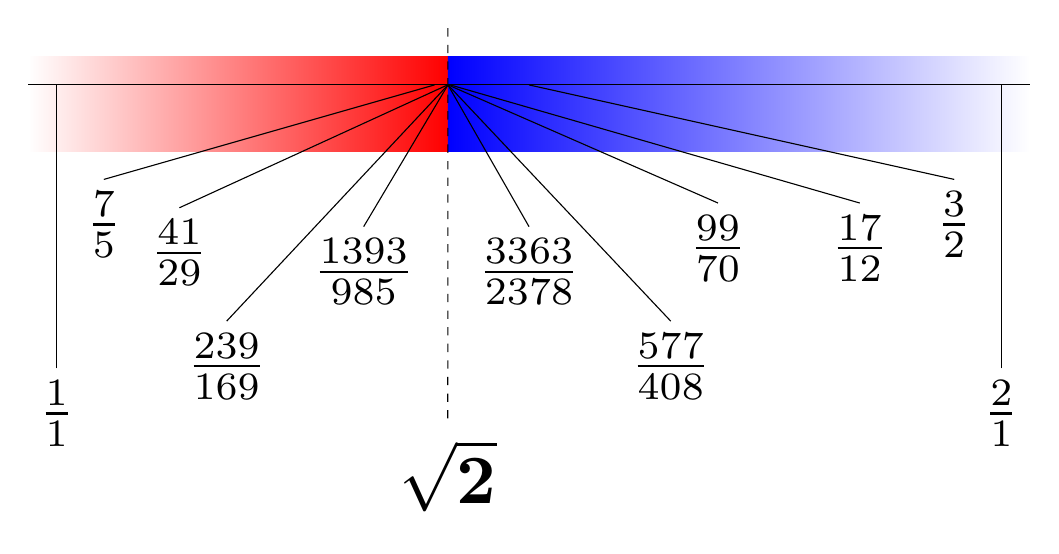
\begin{tikzpicture}[scale = 12, every node/.style={scale=2,inner sep=2pt}]
  \def\sqrtTwo{2^0.5}
  %% 两块渐变区域
  \shade[left color=white, right color=red] (0.97,-0.07) rectangle (\sqrtTwo,0.03);
  \shade[left color=blue, right color=white] (\sqrtTwo,-0.07) rectangle (2.03,0.03);
  %% 数轴
  \draw (0.97,0) -- (2.03,0);
  %% \sqrt{2} 与虚线
  \node[below,scale=1.25] at (\sqrtTwo,-0.36) (nsqrt2) {$\mathbf{\sqrt{2}}$};
  \draw[dashed] (\sqrtTwo, 0.06) -- (nsqrt2);
  %% 其它数字与实线
  \def\nlist{%
    {1/1/(1,-0.3)},%
    {7/5/(1.05,-0.1)},%
    {41/29/(1.13,-0.13)},%
    {239/169/(1.18,-0.25)},%
    {1393/985/(1.325,-0.15)},%
    {3363/2378/(1.5,-0.15)},%
    {577/408/(1.65,-0.25)},%
    {99/70/(1.7,-0.125)},%
    {17/12/(1.85,-0.125)},%
    {3/2/(1.95,-0.1)},%
    {2/1/(2,-0.3)}%
  }
  \foreach \nume / \deno / \pos in \nlist {
    \node[below] at \pos {$\frac{\nume}{\deno}$};
    \draw \pos -- (\nume/\deno,0);
  }
\end{tikzpicture}
%% \end{document}
